\documentclass[tikz,border=8pt]{standalone}
\usepackage{amsmath}
\usetikzlibrary{arrows.meta}
\definecolor{ink}{HTML}{21352F}
\definecolor{teal}{HTML}{087F7B}
\definecolor{blue}{HTML}{4B77A8}
\definecolor{gold}{HTML}{C58B2A}
\definecolor{rose}{HTML}{B65A62}
\begin{document}
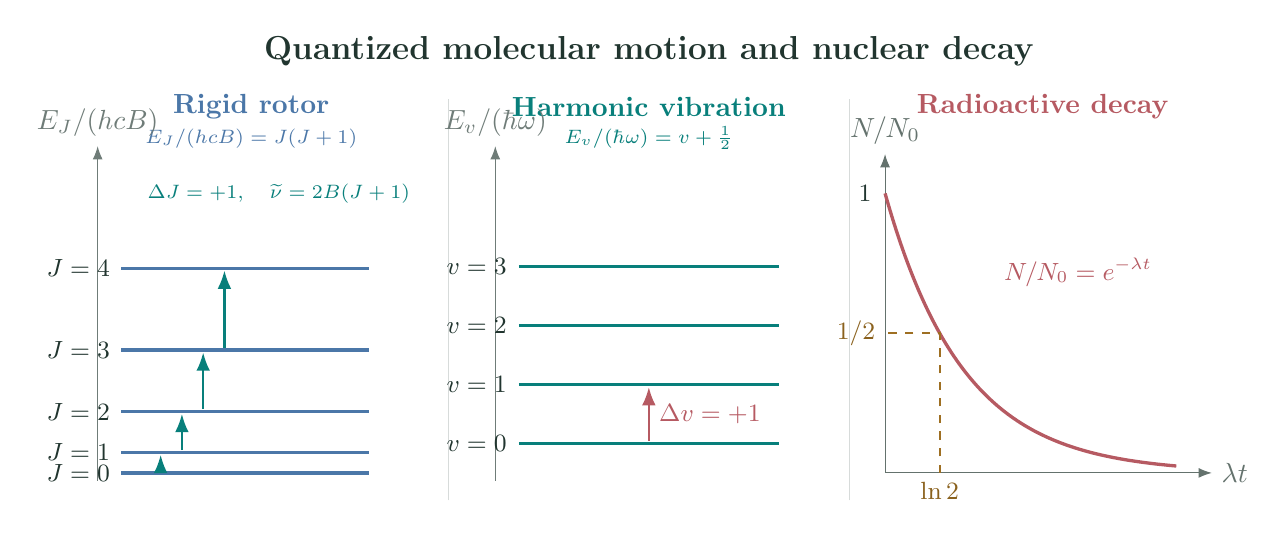
\begin{tikzpicture}[font=\sffamily,text=ink,>=Latex]
  \node[font=\bfseries\large] at (0,5.35)
    {Quantized molecular motion and nuclear decay};

  \node[font=\bfseries,text=blue] at (-5.05,4.65)
    {Rigid rotor};
  \node[font=\scriptsize,text=blue] at (-5.05,4.25)
    {$E_J/(hcB)=J(J+1)$};
  \draw[->,ink!65] (-7.0,-.1)--(-7.0,4.15) node[above] {$E_J/(hcB)$};
  \foreach \J in {0,...,4}{
    \pgfmathsetmacro{\yy}{0.13*\J*(\J+1)}
    \draw[blue,very thick] (-6.7,\yy)--(-3.55,\yy);
    \node[left,font=\small] at (-6.72,\yy) {$J=\J$};
  }
  \foreach \J in {0,...,3}{
    \pgfmathtruncatemacro{\K}{\J+1}
    \pgfmathsetmacro{\ya}{0.13*\J*(\J+1)}
    \pgfmathsetmacro{\yb}{0.13*\K*(\K+1)}
    \draw[teal,->,thick] ({-6.2+0.27*\J},\ya+.03)--
      ({-6.2+0.27*\J},\yb-.03);
  }
  \node[font=\scriptsize,text=teal] at (-4.7,3.55)
    {$\Delta J=+1,\quad\widetilde\nu=2B(J+1)$};

  \draw[ink!18] (-2.55,-.35)--(-2.55,4.75);
  \node[font=\bfseries,text=teal] at (0,4.65)
    {Harmonic vibration};
  \node[font=\scriptsize,text=teal] at (0,4.25)
    {$E_v/(\hbar\omega)=v+\tfrac12$};
  \draw[->,ink!65] (-1.95,-.1)--(-1.95,4.15)
    node[above] {$E_v/(\hbar\omega)$};
  \foreach \v in {0,...,3}{
    \pgfmathsetmacro{\yy}{0.75*(\v+0.5)}
    \draw[teal,very thick] (-1.65,\yy)--(1.65,\yy);
    \node[left,font=\small] at (-1.68,\yy) {$v=\v$};
  }
  \draw[rose,->,thick] (0,.41)--(0,1.09)
    node[midway,right,font=\small] {$\Delta v=+1$};

  \draw[ink!18] (2.55,-.35)--(2.55,4.75);
  \node[font=\bfseries,text=rose] at (5.0,4.65)
    {Radioactive decay};
  \draw[->,ink!70] (3.0,0)--(7.15,0) node[right] {$\lambda t$};
  \draw[->,ink!70] (3.0,0)--(3.0,4.05) node[above] {$N/N_0$};
  \draw[rose,very thick,domain=0:3.7,samples=120,smooth,variable=\x]
    plot ({3.0+\x},{3.55*exp(-\x)});
  \node[left,font=\small] at (2.95,3.55) {$1$};
  \pgfmathsetmacro{\xh}{ln(2)}
  \draw[gold!80!black,dashed,thick]
    ({3+\xh},0)--({3+\xh},{3.55/2})--(3,{3.55/2});
  \node[below,font=\small,text=gold!70!black] at ({3+\xh},0)
    {$\ln2$};
  \node[left,font=\small,text=gold!70!black] at (3,{3.55/2})
    {$1/2$};
  \node[font=\small,text=rose] at (5.45,2.55)
    {$N/N_0=e^{-\lambda t}$};
\end{tikzpicture}
\end{document}
